\section{Datos y el hallazgo de los regímenes}\label{sec:datos}

Hay 197 parcelas en nueve municipios, 138 de entrenamiento y 59 de predicción. FIRA hizo la partición al azar y
estratificada por zona, así que cada municipio con parcelas por predecir también tiene parcelas de entrenamiento. De
las series de tiempo construimos 91 variables por parcela, como el máximo del índice de vegetación NDVI
en 2025, la fenología~\cite{zadoks1974}, la historia de 2022 a 2024, la heterogeneidad dentro de la parcela, el clima y
la topografía. Ninguna usa el rendimiento.

\textbf{Dos maneras de reportar el rendimiento.} Al revisar las etiquetas encontramos dos maneras de reportar el
rendimiento, y cada municipio usa una sola (Fig.~\ref{fig:regimenes}). En cuatro municipios el rendimiento viene con
dos decimales y promedia 4.49\,t/ha. Lo llamamos régimen A. En los otros cinco todos los valores de entrenamiento
tienen un decimal y promedian 3.05\,t/ha. De las 51 etiquetas de este grupo, 44 son múltiplos de 0.5 y las otras 7, de
Singuilucan, solo de 0.1. Lo llamamos régimen B. Por los decimales no sabemos si el rendimiento se midió de forma
distinta o solo se anotó de forma distinta. FIRA nos confirmó que la fuente es mixta, con una comercializadora como
fuente mayoritaria y el productor como la otra, que la báscula no ajusta por humedad y que debemos tratar todos los
registros como una misma variable objetivo. Tampoco conocemos la fuente de cada parcela. Por eso describimos el régimen
como una observación por municipio. La fuente mixta es una posible explicación, pero no podemos confirmarla.

\textbf{Cómo asignamos el régimen.} El régimen es una regla fija por nombre de municipio (Cuadro~\ref{tab:municipios}).
Una vez fijada, no se recalcula en la validación y no usa el rendimiento de la parcela evaluada. No lo asignamos por el
formato de cada etiqueta, porque 7 de las 87 parcelas del régimen A tienen un solo decimal y una regla por formato las
habría mandado al B. Sí fijamos la regla observando las etiquetas de entrenamiento. En seis parcelas de municipios con
una a tres parcelas de entrenamiento (Tepeapulco, Apan, Nanacamilpa y Emiliano Zapata), el régimen se dedujo de su
propia etiqueta y de la cercanía a municipios vecinos con el mismo formato. Sin esas seis parcelas el RMSE de la
validación pasa de 0.458 a 0.464\,t/ha, así que el efecto es pequeño, pero lo reconocemos como un supuesto de diseño.
Las 59 parcelas por predecir pertenecen a municipios que ya tienen al menos una parcela de entrenamiento. El caso más
delicado es el de la parcela de Nanacamilpa, cuyo régimen se apoya en una sola etiqueta.

\begin{table}[t]
\centering
\caption{Parcelas por municipio y régimen.}
\label{tab:municipios}
\footnotesize
\begin{tabular}{@{}llrr@{}}
\toprule
Municipio & Régimen & Entrenamiento & Predicción \\
\midrule
Chignahuapan & A & 71 & 29 \\
Almoloya & A & 10 & 4 \\
Cuautepec de Hinojosa & A & 5 & 4 \\
Tepeapulco & A & 1 & 0 \\
Calpulalpan & B & 30 & 14 \\
Singuilucan & B & 16 & 7 \\
Emiliano Zapata & B & 3 & 0 \\
Apan & B & 1 & 0 \\
Nanacamilpa & B & 1 & 1 \\
\midrule
Total A, B & & 87, 51 & 37, 22 \\
\bottomrule
\end{tabular}
\end{table}

\begin{figure}[t]
\centering
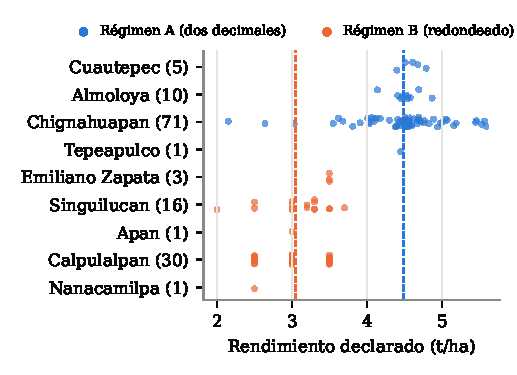
\includegraphics[width=\columnwidth]{f1_regimenes}
\caption{Rendimiento declarado de las 138 parcelas de entrenamiento por municipio, con el número de parcelas entre
paréntesis. Las líneas punteadas son la media de cada régimen.}
\label{fig:regimenes}
\end{figure}

Este hallazgo cambia el problema. La diferencia entre las medias de los regímenes, de 1.4\,t/ha, es casi tres veces la
desviación estándar dentro de cada uno (0.53\,t/ha en A y 0.40 en B). Además, el redondeo de las etiquetas del régimen B
limita lo que cualquier modelo puede predecir. Si el valor verdadero se redondeó a 0.5\,t/ha y se distribuye de forma
uniforme dentro del intervalo de redondeo, el redondeo agrega una desviación de $0.5/\sqrt{12}=0.14$\,t/ha. Esto es una
cota aproximada y no un error mínimo obligatorio, porque 7 de las 51 etiquetas tienen un paso de 0.1. Con la mezcla
observada de pasos la cota es 0.134 y, si todas tuvieran paso de 0.1, sería 0.029. Por el tamaño de la diferencia entre
regímenes, el régimen es la primera pieza del modelo.
